\documentclass[conference]{IEEEtran}
\IEEEoverridecommandlockouts

% --- Packages -------------------------------------------------------------
\usepackage{cite}
\usepackage{amsmath}
\usepackage{newtxtext}   % Times text, the professional IEEE look
\usepackage{newtxmath}   % matching Times math (loaded after amsmath)
\usepackage{array}
\usepackage{booktabs}
\usepackage{url}
\usepackage{xcolor}
\usepackage{tikz}
\usetikzlibrary{arrows.meta,positioning,calc}
\usepackage{pgfplots}
\pgfplotsset{compat=1.18}
\usepackage[hidelinks]{hyperref}

% No automatic end-of-line hyphenation. Lines stay justified and avoid overfull
% boxes through micro-stretch rather than by breaking words with a hyphen.
\hyphenpenalty=10000
\exhyphenpenalty=10000
\tolerance=9999
\emergencystretch=3em

% IEEEtran prints "Abstract" and "Index Terms" followed by an em dash. Replace that
% separator with a colon so no dash appears in the running text.
\usepackage{etoolbox}
\patchcmd{\abstract}{\textit{\abstractname}---\relax}{\textit{\abstractname}:\ }{}{}
\patchcmd{\IEEEkeywords}{\textit{\IEEEkeywordsname}---\relax}{\textit{\IEEEkeywordsname}:\ }{}{}

% TikZ styles shared by the figures.
\tikzset{
  lbox/.style={draw, rounded corners=2pt, align=center, font=\scriptsize,
               text width=17mm, minimum height=9mm, inner sep=2pt, fill=blue!5},
  iobox/.style={lbox, fill=black!8},
  cbox/.style={lbox, fill=green!8},
  stepbox/.style={draw, rounded corners=2pt, align=center, font=\scriptsize,
               text width=58mm, minimum height=6mm, inner sep=3pt, fill=blue!5},
  flow/.style={-{Latex[length=2mm]}, semithick},
}

\newcommand{\code}[1]{\texttt{\small #1}}

\begin{document}

\title{Lattice: Signed, Replayable Capability Receipts for Model Runs}

\author{\IEEEauthorblockN{Lakshman Turlapati}
\IEEEauthorblockA{Full Self Browsing\\
Email: lakshmanturlapati@gmail.com\\
Code: \url{https://github.com/fullselfbrowsing/Lattice}}}

\maketitle

% --- Abstract -------------------------------------------------------------
\begin{abstract}
Production systems built on large language models increasingly route work across
many providers and modalities, yet the run itself remains opaque. A typical stack
records, at best, a free text log that no third party can verify and no operator
can replay. We present Lattice, a capability first TypeScript runtime in which
every model run emits a \emph{capability receipt}: a canonical, signed, and
replayable record of what the system was asked to do, how it routed the work, what
constraints it enforced, and what it produced. A receipt is canonicalized with the
JSON Canonicalization Scheme (RFC 8785), redacted before signing so that no secret
ever enters the signed bytes, and signed with Ed25519 inside a Dead Simple Signing
Envelope. Routing is a deterministic and inspectable pure function rather than an
opaque model call, output invariants carry terminal semantics so a violated run is
never silently retried, and a verifier can reconstruct the run offline and confirm
that the recomputed output hash matches the signed receipt. We describe the threat
model, the design of the receipt and replay pipeline, and an implementation that
ships as two published npm packages with 960 automated tests across 82 files, a
seven provider parity contract, and a content addressed command line tool for
reproduction and verification. Our evaluation is assurance by construction: the
guarantees are expressed as code level invariants and property tests rather than as
a latency benchmark. The result is a small runtime that makes auditability and
reproducibility a default property of every multimodal model run.
\end{abstract}

\begin{IEEEkeywords}
capability receipts, verifiable replay, LLM orchestration, software supply chain,
canonical JSON, digital signatures, reproducibility, multimodal AI
\end{IEEEkeywords}

% --- Introduction ---------------------------------------------------------
\section{Introduction}

Software that calls large language models has moved from prototypes into systems
that approve refunds, triage insurance claims, route field operations, and process
medical and recruiting documents. These systems combine text with images, audio,
documents, structured outputs, and tool calls, and they increasingly spread a
single task across several model providers for cost, latency, privacy, or
capability reasons. As the stakes rise, two questions follow every run. First, can
an operator or an auditor trust the record of what happened. Second, can anyone
reproduce that run later, offline, without trusting the party that produced the
record. Today the honest answer to both questions is usually no.

The reason is structural. The dominant integration libraries are provider wrappers.
They normalize the shape of a chat or generation call across vendors and they
provide convenience around tools, memory, and agents. They do not produce a
tamper evident record of a run, they do not commit to a deterministic and
inspectable account of why one model was chosen over another, and they do not let a
third party replay the run and check the result against a signed artifact. A free
text log is not a proof. It can be edited after the fact, it does not bind the
inputs to the outputs, and it carries no signature that a verifier can check with a
public key.

This paper argues that the missing primitive is a per run, signed, replayable
\emph{capability receipt}, and that a runtime can make such a receipt a default
byproduct of normal operation rather than an after the fact instrumentation task.
We build this argument concretely through Lattice, a capability first runtime SDK
written in TypeScript. A developer describes the job, supplies any mix of artifacts,
declares the desired outputs and policy constraints, and optionally attaches a
contract. Lattice then routes the work deterministically, packs context, prepares
artifacts for the chosen provider, enforces output invariants, and emits a receipt
on every outcome, success or failure.

Lattice provides four guarantees that together make a run auditable and
reproducible.

\begin{enumerate}
\item \textbf{Deterministic and inspectable routing.} The router is a pure function
of the capability catalog, the request, and the policy. It uses hard filters, a
stable score, and a deterministic tie break, and it reports the full set of
candidates, the rejected candidates, the fallback chain, and a typed list of reasons
when no route is possible. There is no randomness and no model call inside routing.
\item \textbf{Terminal output invariants.} Output level tripwires such as
``must cite an artifact'' or ``no personally identifiable information'' are evaluated
by a pure kernel. A violation produces a terminal error that the fallback chain is
forbidden to retry, which prevents a system from quietly trying again until a banned
output slips through.
\item \textbf{Signed capability receipts.} Every run emits a receipt that is
canonicalized with RFC 8785, redacted before signing, and signed with Ed25519 inside
a Dead Simple Signing Envelope. The receipt binds the run record to a key through a
signature that any holder of the public key can check.
\item \textbf{Offline verifiable replay.} A receipt and its content addressed
artifacts can be materialized into a replay envelope. Materialization verifies the
signature before it loads any artifact, and a property test confirms that
reconstructing the run and recomputing the output hash yields the value committed in
the receipt.
\end{enumerate}

We make the following contributions. We define the capability receipt as a signing
and replay primitive for multimodal model runs, and we show how a redact then sign
ordering and a canonical encoding turn it into a verifiable artifact rather than a
log line. We show how a deterministic and inspectable router, terminal output
invariants, and a content addressed verification tool compose into a runtime where
auditability and reproducibility are default properties. We describe a working
implementation that ships publicly with supply chain provenance, a seven provider
parity contract, and a test suite that encodes the guarantees as invariants. We
discuss what signed receipts enable in practice and we state plainly what they do
not provide. The remainder of the paper covers background and related work, the
threat model and goals, the design, the implementation, the evaluation, a
discussion, the limitations, future work, and a conclusion.

% --- Background and Related Work ------------------------------------------
\section{Background and Related Work}

\subsection{Provider wrappers and agent frameworks}

A first family of systems normalizes model access. The Vercel AI SDK
\cite{vercelaisdk} offers a broad provider agnostic TypeScript toolkit with
multimodal generation, tools, and agents. LangChain and LangGraph \cite{langchain}
provide orchestration, sessions, and tracing. LiteLLM \cite{litellm} is strong
routing infrastructure that exposes a common interface across many providers with
fallback and gateway features. The OpenAI Agents SDK \cite{openaiagents} provides
agent loops, sessions, and tool use. The Model Context Protocol \cite{mcp}
standardizes how tools and context attach to a model session. These systems are
valuable and widely used. None of them, however, emit a signed and replayable per
run receipt. Their tracing is observability for humans, not a cryptographic artifact
that a third party can verify against a public key, and their routing is generally
either configuration driven or model chosen rather than a deterministic pure
function whose full decision is recorded.

\subsection{Software supply chain provenance}

A second family secures the provenance of software artifacts. in-toto
\cite{intoto} provides end to end guarantees over a software supply chain by signing
the steps that produced an artifact. The Dead Simple Signing Envelope \cite{dsse}
defines a minimal envelope and a pre authentication encoding so that signatures
commit unambiguously to a payload and its type. Sigstore \cite{sigstore} makes
signing and transparency broadly accessible. SLSA \cite{slsa} defines levels of
supply chain integrity, and The Update Framework \cite{tuf} addresses survivable key
compromise in update systems. Lattice borrows directly from this lineage. It reuses
the DSSE envelope and pre authentication encoding, it adopts a key set with explicit
key states in the spirit of key rotation and revocation, and it treats the published
package itself as a supply chain artifact with provenance attestations. The novelty
is to apply this provenance discipline not to a build, but to an individual model run
at runtime.

\subsection{Canonicalization and signatures}

Signing a structured object requires a deterministic byte encoding, otherwise two
semantically equal objects can produce different signatures. The JSON Canonicalization
Scheme \cite{rfc8785} defines such an encoding for JSON, and the I-JSON message format
\cite{rfc7493} constrains JSON to an interoperable subset, which matters for how
numbers and floats are serialized. Lattice canonicalizes receipts with RFC 8785 and
serializes monetary cost as an I-JSON string so that receipts never carry raw floats.
Signatures use EdDSA \cite{rfc8032}, the elliptic curve signature construction that is
widely deployed for compact and fast signatures.

\subsection{Transparency and reproducibility in machine learning}

A third family documents models and data for accountability. Model Cards
\cite{modelcards} and Datasheets for Datasets \cite{datasheets} standardize
disclosure about a model or dataset, and reproducibility programs in the research
community \cite{reproml} push toward runs that others can repeat. These efforts
describe an artifact or a study. A capability receipt is complementary and finer
grained. It describes a single production run and makes that run independently
checkable and replayable. Merkle trees \cite{merkle} provide a standard way to commit
to a set of items with a single root, which we identify as the natural mechanism for
a future signed lineage root over the artifacts that a run consumed and produced.

\subsection{The gap}

Across these families, no system provides a per run, signed, canonical, and offline
replayable receipt for multimodal model work, backed by a deterministic and
inspectable router and by output invariants with terminal semantics. Lattice
occupies that gap.

% --- Threat Model and Goals -----------------------------------------------
\section{Threat Model and Goals}

\subsection{Actors and trust assumptions}

We consider four actors. The \emph{issuer} is the Lattice runtime that performs a
run and signs a receipt with a private key. The \emph{provider} is an external model
service that the runtime calls and that we treat as untrusted and possibly buggy. The
\emph{verifier} is any party that later receives a receipt and wishes to check it,
possibly without trusting the issuer at the time of verification. The
\emph{adversary} may sit between these actors or may hold material that looks
legitimate.

\subsection{Adversary capabilities}

We assume an adversary who can tamper with a stored receipt, a transcript, or a
claimed output after a run completes. We assume an adversary who can attempt to
substitute a different model route while presenting a receipt that attests to the
intended route. We consider an adversary who has obtained a valid signing key and who
then tries to mint a receipt in an older schema in order to bypass integrity fields
that newer schemas commit to, a schema downgrade attack. We also consider a careless
issuer whose run inputs contain secrets or personally identifiable information that
must never be embedded in a signed and shareable artifact.

\subsection{Security goals}

The runtime targets five goals. First, integrity of the run record: a receipt that
has been altered must fail verification. Second, non repudiation through signature:
a verifier with the public key can confirm which key signed a receipt and whether
that key is active, retired, or revoked. Third, redaction before signing: secrets and
detected personally identifiable information are removed from the body before the
canonical bytes are produced, so they never enter the signature and never travel with
the receipt. Fourth, determinism for replay: a verifier can recompute the output hash
from the reconstructed run and compare it to the value the receipt commits to. Fifth,
downgrade resistance: a receipt in a superseded schema is rejected before any
cryptographic work, so possession of a valid key is not sufficient to evade newer
schema commitments.

\subsection{Non goals}

Several properties are explicitly out of scope. We do not provide confidentiality of
provider traffic, which is the responsibility of transport security. We do not
reproduce the live behavior of a remote model, since model providers are
nondeterministic and outside our trust boundary. Replay reconstructs the recorded run
and its output hash, not a fresh call to the provider. We also do not operate a hosted
control plane. Lattice is a runtime SDK, and the receipt is a portable artifact that
travels with the run rather than a record locked inside a service.

% --- Design ---------------------------------------------------------------
\section{Design}

Figure~\ref{fig:arch} shows the end to end run lifecycle that produces and then
consumes a capability receipt. The subsections that follow walk through each stage.

\begin{figure*}[t]
\centering
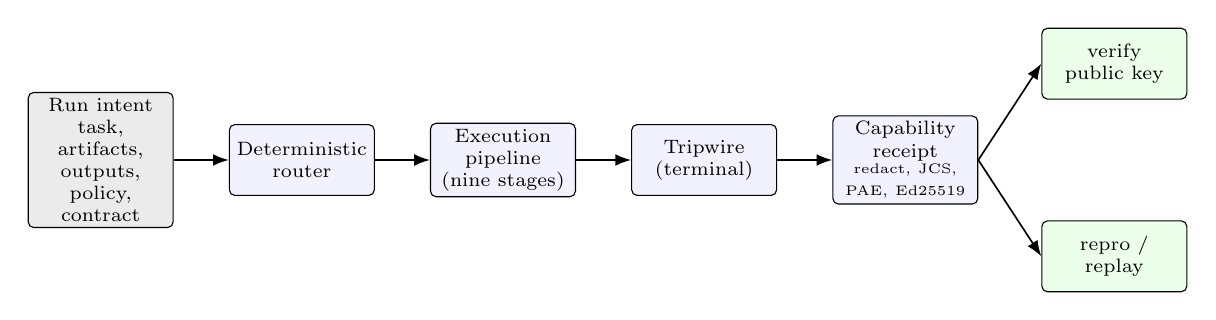
\begin{tikzpicture}[node distance=6mm and 7mm]
  \node[iobox] (intent) {Run intent\\ task, artifacts,\\ outputs, policy,\\ contract};
  \node[lbox, right=of intent] (router) {Deterministic\\ router};
  \node[lbox, right=of router] (exec) {Execution\\ pipeline\\ (nine stages)};
  \node[lbox, right=of exec] (trip) {Tripwire\\ (terminal)};
  \node[lbox, right=of trip] (rcpt) {Capability\\ receipt\\ \tiny redact, JCS,\\ \tiny PAE, Ed25519};
  \node[cbox, above right=2mm and 8mm of rcpt] (verify) {verify\\ public key};
  \node[cbox, below right=2mm and 8mm of rcpt] (repro) {repro /\\ replay};
  \draw[flow] (intent) -- (router);
  \draw[flow] (router) -- (exec);
  \draw[flow] (exec) -- (trip);
  \draw[flow] (trip) -- (rcpt);
  \draw[flow] (rcpt.east) -- (verify.west);
  \draw[flow] (rcpt.east) -- (repro.west);
\end{tikzpicture}
\caption{The Lattice run lifecycle. A run intent is routed by a deterministic and
inspectable function, executed through a nine stage pipeline, checked by terminal
output invariants, and committed to a signed capability receipt. The receipt is later
consumed by offline verification and by content addressed reproduction.}
\label{fig:arch}
\end{figure*}

\subsection{The capability first run model}

A run is described by a small intent: a \code{task} string, a set of \code{artifacts}
that may be text, JSON, images, audio, documents, or tool results, a map of declared
\code{outputs} with their schemas, a \code{policy} that expresses privacy, latency,
provider allow and deny lists, and budget, and an optional \code{contract}. The
developer does not select a model. The runtime selects one from a capability catalog
and records the decision. This capability first shape is what makes a receipt
meaningful, because the receipt can record the declared intent and the chosen route
side by side.

\subsection{Deterministic and inspectable routing}

Routing is implemented as a pure function, \code{routeDeterministically}, that takes
the capability catalog, the request, and the policy and returns a route decision. It
performs no input or output, draws no randomness, and never calls a model. The
function first applies hard filters that reject a candidate when the provider is
unavailable, when an explicit provider or model override does not match, when a
required input or output modality is unsupported, when structured output is required
but unsupported, or when the estimated input exceeds the context window. It then
applies policy filters that reject on an allow or deny list, on a privacy class, on a
no logging or no upload requirement, on a latency class, or on a budget ceiling.
Surviving candidates are scored from cost, latency, context headroom, and catalog
index, and ties are broken by a stable order over acceptance status, score, provider
name, and model name. The decision exposes the selected route, all candidates, all
rejected candidates, a fallback chain of policy preserving alternatives, and a
deduplicated list of typed reasons when no route is possible. The full execution plan
is stable JSON with a nine stage pipeline: analysis, transforms, context packing,
provider packaging, tool execution, execution, validation, tripwire, and persistence.
Because the decision is a pure function and is recorded in full, the receipt can
attest to exactly why a model was chosen, and a reviewer can reproduce the decision
by re running the function on the same inputs.

\subsection{Output invariants with terminal semantics}

Lattice lets a developer attach output invariants through a fluent builder,
\code{inv}, with constructors \code{mustCite}, \code{fieldFromTable}, \code{noPII},
and \code{matches}, where the last validates against a Standard Schema
\cite{standardschema}. These invariants are evaluated by a pure kernel,
\code{evaluateTripwires}, that performs no input or output, reads no clock, and uses
no randomness, so the same output and the same invariants always yield the same
result. The kernel aborts on the first violation. The default detector set for
\code{noPII} contains four detectors: email, United States social security number,
credit card validated by the Luhn checksum, and United States phone number. When a no
personally identifiable information invariant fires, the evidence is redacted to the
detector name and the matched substring, so the violating secret is not copied into
the evidence. A violation produces a \code{TripwireViolationError} that carries the
flag \code{terminal: true}. The predicate \code{isTerminal} returns true for a
tripwire violation and for a no contract match, and the fallback chain consults this
predicate so that a terminal failure is never retried. This matters for safety: a
system that retries until a banned output passes is worse than a system that fails
closed, and terminal semantics make failing closed the default.

\subsection{Capability contracts and preflight}

A contract expresses requirements that must hold before and around a run: a budget
with a maximum cost and, for agent runs, iteration and wall time caps, a set of
invariants, a quality floor, a set of required modalities, and a required privacy
class. A pure preflight evaluator, \code{evaluateContractAgainstRoute}, runs inside
the router and can reject a route with a typed reason such as a budget exceeded, a
missing modality, or a privacy mismatch. A quality floor reason is reserved for the
evaluation tool described later. Usage is normalized to prompt tokens, completion
tokens, and a cost in United States dollars on every outcome, success or failure, and
a null cost is distinct from a zero cost so that an unmeasured price is never confused
with a free call.

\subsection{The capability receipt}

The receipt is the central artifact. Its construction enforces a strict ordering that
is the heart of the security argument. Figure~\ref{fig:pipeline} shows the pipeline,
and Figure~\ref{fig:envelope} shows the resulting envelope.

First, the runtime assembles the raw receipt body from the run record. Second, it
redacts the body. Redaction removes secrets and detected personally identifiable
information and records a manifest of redactions, each with a path and a reason, and a
signed redaction policy identifier whose default value is \code{lattice.default.v1}.
Third, it canonicalizes the redacted body with RFC 8785 \cite{rfc8785}. Fourth, it
base64 encodes the canonical bytes as the payload. Fifth, it builds the DSSE pre
authentication encoding over the payload type and the payload. Sixth, it signs the
pre authentication encoding with Ed25519. The ordering is enforced structurally, not
by convention: the canonicalization function is only ever called on the output of the
redaction function, so a code path that signs unredacted bytes is unrepresentable.
This is what we mean by redact then sign as an architectural invariant rather than a
guideline.

\begin{figure}[t]
\centering
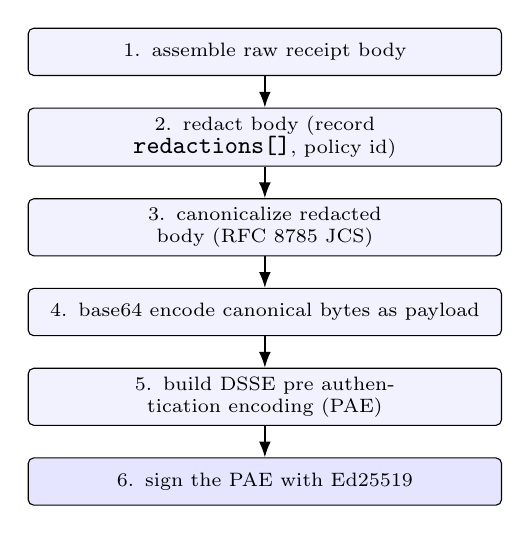
\begin{tikzpicture}[node distance=4mm]
  \node[stepbox] (s1) {1. assemble raw receipt body};
  \node[stepbox, below=of s1] (s2) {2. redact body (record \code{redactions[]}, policy id)};
  \node[stepbox, below=of s2] (s3) {3. canonicalize redacted body (RFC 8785 JCS)};
  \node[stepbox, below=of s3] (s4) {4. base64 encode canonical bytes as payload};
  \node[stepbox, below=of s4] (s5) {5. build DSSE pre authentication encoding (PAE)};
  \node[stepbox, below=of s5, fill=blue!10] (s6) {6. sign the PAE with Ed25519};
  \draw[flow] (s1) -- (s2);
  \draw[flow] (s2) -- (s3);
  \draw[flow] (s3) -- (s4);
  \draw[flow] (s4) -- (s5);
  \draw[flow] (s5) -- (s6);
\end{tikzpicture}
\caption{The receipt construction pipeline. Canonicalization is only ever applied to
the output of redaction, so signing unredacted bytes is structurally impossible.}
\label{fig:pipeline}
\end{figure}

\begin{figure}[t]
\centering
\scriptsize
\begin{verbatim}
{
  "payloadType":
    "application/vnd.lattice.receipt+json",
  "payload": "<base64(JCS(redacted body))>",
  "signatures": [
    { "keyid": "<kid>",
      "sig": "<base64(Ed25519(PAE))>" }
  ]
}
\end{verbatim}
\caption{The Dead Simple Signing Envelope produced for a receipt. The pre
authentication encoding concatenates the literal \code{DSSEv1}, the payload type and
its length, and the payload and its length, all in a fixed order.}
\label{fig:envelope}
\end{figure}

The signing key is identified by a \code{kid} and resolved through a key set. A key
set maps a \code{kid} to a key entry whose state is \emph{active}, \emph{retired}, or
\emph{revoked}. Cost is serialized as an I-JSON \cite{rfc7493} string or null so that
receipts never carry raw floating point numbers. The signature is computed over the
pre authentication encoding rather than over the raw JSON, which removes any ambiguity
about what the signature commits to.

\subsection{Schema versioning and downgrade defense}

Receipts carry an explicit version. Three versions exist: \code{lattice-receipt/v1},
\code{lattice-receipt/v1.1}, and \code{lattice-receipt/v1.2}. The v1.2 schema adds an
optional and signed model class field that records the training class of the chosen
model. Verification rejects a body whose version is the original v1 or is absent, with
the error \code{schema-version-too-low}, and it does so before any cryptographic work.
This is the downgrade defense from the threat model. An adversary who holds a valid
signing key still cannot mint a v1 shaped body to evade the integrity fields that the
v1.1 and v1.2 schemas commit to, because the structural version check fails first.

\subsection{Verification}

Verification, \code{verifyReceipt}, returns a result that is either an ok value with
the verified body and the resolved key state, or a failure value with a typed error.
There are exactly seven error kinds, listed in Table~\ref{tab:verify}. Verification
checks the envelope shape, the schema version, the key existence and state, the
re canonicalization match, and finally the Ed25519 signature, with a defense in depth
check that the \code{kid} inside the body matches the key entry.

\begin{table}[t]
\centering
\caption{The seven \code{verifyReceipt} error kinds.}
\label{tab:verify}
\scriptsize
\begin{tabular}{@{}l p{0.47\columnwidth}@{}}
\toprule
Error kind & Fires when \\
\midrule
\code{envelope-malformed} & the envelope cannot be decoded or has no signatures \\
\code{version-mismatch} & the body shape or version is unknown \\
\code{schema-version-too-low} & the body is v1 or has no version (downgrade defense) \\
\code{key-not-found} & the \code{kid} is not in the key set \\
\code{key-revoked} & the resolved key is in the revoked state \\
\code{canonicalization-mismatch} & the re canonicalized body differs from the signed bytes \\
\code{signature-invalid} & the Ed25519 check fails or the body \code{kid} mismatches \\
\bottomrule
\end{tabular}
\end{table}

\subsection{Offline verifiable replay}

A receipt becomes useful for reproduction through replay. A replay envelope carries
optional receipt and contract fields. The function \code{materializeReplayEnvelope}
reconstructs a replay envelope from a receipt and a set of content addressed
artifacts, and it enforces a critical ordering: it verifies the receipt before it
loads any artifact. A test confirms that the artifact loader is called zero times when
verification fails, which prevents a tampered receipt from causing artifact loads or
side effects. Materialization can fail with one of three kinds:
\code{verify-failed}, \code{artifact-load-failed}, and \code{envelope-malformed}. A
property test asserts that the round trip from \code{createReceipt} through
\code{materializeReplayEnvelope} through \code{replayOffline} preserves the output
hash, which is the concrete statement of the determinism goal.

\subsection{The four guarantees and their enforcement}

Table~\ref{tab:guarantees} maps each guarantee to the mechanism that provides it and
to the property or test that enforces it. The point of the table is that none of the
guarantees rest on a convention or a comment. Each is enforced by structure or checked
by a test that fails the build when the property is violated.

\begin{table}[t]
\centering
\caption{Each guarantee, its mechanism, and its enforcement.}
\label{tab:guarantees}
\footnotesize
\begin{tabular}{@{}p{0.27\columnwidth} p{0.31\columnwidth} p{0.30\columnwidth}@{}}
\toprule
Guarantee & Mechanism & Enforcement \\
\midrule
Deterministic routing & a pure routing function & recorded decision, no I/O or randomness \\
Terminal invariants & \code{isTerminal} consulted by fallback & fallback never retries a terminal error \\
Redact then sign & canonicalize only on redaction output & ordering is structurally unrepresentable otherwise \\
Verifiable replay & verify before load & loader call count is zero on verify failure; output hash round trip \\
\bottomrule
\end{tabular}
\end{table}

% --- Implementation -------------------------------------------------------
\section{Implementation}

\subsection{Packaging and footprint}

Lattice is a TypeScript pnpm workspace that publishes two packages,
\code{@full-self-browsing/lattice} and \code{@full-self-browsing/lattice-cli}, both at
version 1.3.0. The packages are live on the public npm registry. They are published
with an OpenID Connect trusted publisher and with supply chain provenance attestations
in the spirit of SLSA \cite{slsa}, and a tagged GitHub release accompanies the
publish. The runtime targets Node version 24 or newer. The implementation is about
21,584 lines of production TypeScript across the packages. The core package has a
deliberately small runtime dependency surface of three packages: \code{canonicalize}
for RFC 8785 encoding, \code{@standard-schema/spec} for schema contracts, and
\code{mime} for artifact typing. The Ed25519 reference oracle and the schema library
used in tests are development dependencies only, so a consumer of the core package
does not inherit them.

\subsection{Signing internals}

Signing uses the Node 24 WebCrypto interface with the literal algorithm name
\code{Ed25519}. Keys are represented as JSON Web Keys of the octet key pair type and
signatures are 64 bytes as specified by EdDSA \cite{rfc8032}. To guard against a
silent regression in the platform implementation, a development only parity oracle
signs the same message with an independent Ed25519 library and asserts a byte for byte
match in the test suite. The oracle is never on the production signing path.

\subsection{The seven provider parity contract}

Lattice defines seven logical provider adapters: \code{openai},
\code{openai-compatible}, \code{anthropic}, \code{gemini}, \code{xai},
\code{openrouter}, and \code{lm-studio}. An internal invariant named INV-03 states
that every improvement must work equally across all seven universal provider targets.
A parity smoke test makes this concrete. As summarized in Table~\ref{tab:parity}, the
test iterates all seven adapters against provider shaped fake responses and asserts a
uniform adapter shape, string raw outputs, the normalized usage shape, an error on a
non success response, propagation of an abort signal into the underlying fetch, a raw
response pass through, and that the set of adapter identifiers has size seven. The
parity contract is what lets a receipt mean the same thing regardless of which provider
served the run.

\begin{table}[t]
\centering
\caption{What the INV-03 parity smoke test asserts across all seven providers.}
\label{tab:parity}
\footnotesize
\begin{tabular}{@{}p{0.30\columnwidth} p{0.60\columnwidth}@{}}
\toprule
Property & Assertion \\
\midrule
adapter shape & each adapter exposes the same surface \\
raw outputs & content is returned as strings keyed by output name \\
usage shape & normalized prompt and completion tokens and cost \\
error path & a non success response throws with provider identity \\
cancellation & the request abort signal reaches the fetch \\
raw response & the original parsed body is available \\
identity & the set of adapter ids has size seven \\
\bottomrule
\end{tabular}
\end{table}

\subsection{The capability registry}

Routing consults a capability catalog backed by a registry of 332 model profiles. Of
these, 328 are generated from a snapshot of an OpenRouter model feed and 4 are hand
maintained static supplements for direct adapters, namely an Anthropic Opus profile, a
Gemini Pro profile, an LM Studio local template, and an xAI Grok profile. A weekly
continuous integration drift gate guards the generated file so that the catalog does
not silently diverge from the upstream feed. At call time the runtime can refine a
profile through capability negotiation, fetching a live model listing with a time to
live cache and inflight request coalescing, and falling back to the registry on a
transient error. Adapter quirk flags capture provider specific behavior so that the
runtime can adapt without breaking the parity contract.

\subsection{The command line tool}

The \code{lattice} command line tool ships in the second package. It uses a lazily
loaded subcommand structure and a consistent exit code convention of 0 for success, 1
for a verification or test failure, and 2 for a load or configuration failure. Three
subcommands exist today. The \code{verify} subcommand checks the signature and the
structure of a receipt and prints the key identifier and the contract verdict. The
\code{repro} subcommand performs a full content addressed reproduction: it loads the
receipt, verifies it, materializes the replay envelope, replays offline, and diffs the
recomputed output hash, returning 0 on a match and 1 on a drift. The \code{eval}
subcommand walks a directory of receipts, replays each, and gates layered determinism
along with cost and quality regressions relative to a baseline, with a flag to
initialize a fresh baseline and a disk backed judge cache. These three subcommands turn
a receipt from a passive record into an executable regression and audit gate.

\subsection{Agents and chained receipts}

Lattice exposes a runtime agent entry point, \code{ai.runAgent}, that drives a uniform
tool use loop across all seven providers, and an opt in multi agent crew surface,
\code{defineAgent} and \code{runAgentCrew}. A crew shares a budget with structural caps
on total iterations, per agent iterations, concurrent children, and depth, and it
coordinates rate limits through a token bucket with sensible defaults. Crucially, each
child receipt chains to a crew root through a parent receipt content identifier, so a
multi agent run produces a verifiable tree of receipts rather than a single opaque
trace. A helper, \code{evalAgentRun}, gates iterations to goal and cost against a
baseline. Three runnable examples exercise these surfaces end to end: a multimodal work
inbox that demonstrates a contract, a signed receipt, a tripwire violation, and a no
contract match, a single agent loop that emits per iteration checkpoint receipts, and a
crew example that demonstrates chained receipts and an evaluation gate.

% --- Evaluation -----------------------------------------------------------
\section{Evaluation}

Our evaluation is assurance by construction. The claims in this paper are properties of
the system, and we evaluate them by encoding each as an invariant or a property test
that fails the build when the property does not hold, rather than by measuring latency
or model output quality, which depend on providers outside our trust boundary. The
suite contains 960 automated test cases across 82 test files, with 816 in the core
package and 144 in the command line package, and it runs under a standard TypeScript
test runner. Figure~\ref{fig:tests} shows the distribution by package.

\begin{figure}[t]
\centering
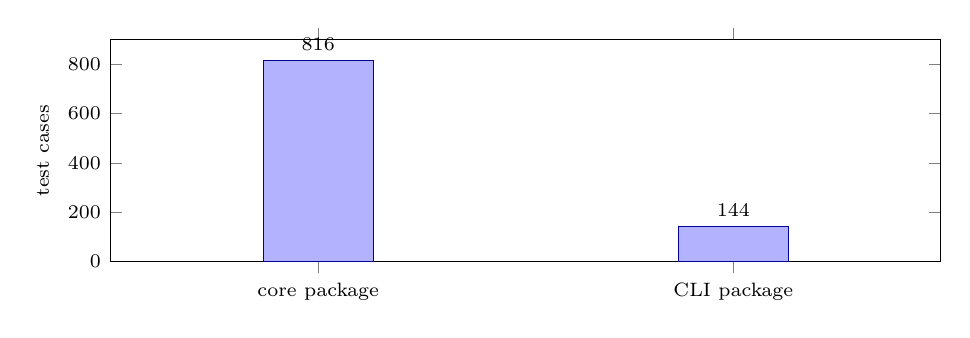
\begin{tikzpicture}
\begin{axis}[
  ybar,
  width=\columnwidth, height=44mm,
  bar width=14mm,
  ymin=0, ymax=900,
  ylabel={test cases},
  ylabel near ticks,
  symbolic x coords={core package, CLI package},
  xtick=data,
  nodes near coords,
  every node near coord/.append style={font=\scriptsize},
  xticklabel style={font=\scriptsize},
  yticklabel style={font=\scriptsize},
  ylabel style={font=\scriptsize},
  enlarge x limits=0.5,
]
\addplot[draw=blue!60!black, fill=blue!30] coordinates {(core package,816) (CLI package,144)};
\end{axis}
\end{tikzpicture}
\caption{Automated test cases by package. The suite totals 960 cases across 82 files,
816 in the core package and 144 in the command line package, and it encodes the
paper's guarantees as executable obligations.}
\label{fig:tests}
\end{figure}

We organize the evaluation around the four guarantees.

\textbf{Determinism of routing and invariants.} The router and the tripwire kernel are
pure functions. Tests assert that the same inputs always produce the same route
decision and the same tripwire result, and the absence of input, output, clock reads,
and randomness in these functions is verified by construction and by review. Because
the decision is recorded in the plan and the receipt, a reviewer can reproduce a route
by re running the function.

\textbf{Redact then sign.} The ordering is structurally enforced because the
canonicalization function is only ever called on the output of the redaction function.
Tests confirm that the redaction manifest and the signed redaction policy identifier
appear in the signed body and that a no personally identifiable information violation
redacts evidence to a detector name and a matched substring.

\textbf{Downgrade resistance and verification.} Tests cover all seven verification
error kinds. In particular, a body in the original v1 schema, or a body with no
version, is rejected with a schema version too low error before any cryptographic work,
which demonstrates the downgrade defense. Tests also confirm that a revoked key yields
a key revoked error and that a mismatch between the body key identifier and the key
entry yields a signature invalid error.

\textbf{Verifiable replay.} A test asserts that the artifact loader is called zero
times when receipt verification fails during materialization, which shows that a
tampered receipt cannot trigger artifact loads. A property test asserts that the round
trip from receipt creation through materialization through offline replay preserves the
output hash, which is the determinism goal stated as a checkable property. The
\code{repro} subcommand exercises the same path end to end and returns a distinct exit
code for a match and for a drift.

\textbf{Parity.} The INV-03 smoke test exercises all seven providers and asserts the
uniform behavior summarized in Table~\ref{tab:parity}, including that the set of
adapter identifiers has size seven. Parity is what lets a single receipt format and a
single verification path apply regardless of which provider served the run.

Taken together, these tests turn the paper's guarantees into executable obligations.
A change that weakens a guarantee fails the suite, so the guarantees are maintained
across the lifetime of the project rather than asserted once.

% --- Discussion -----------------------------------------------------------
\section{Discussion}

Signed capability receipts change what is possible after a run. An operator can hand a
receipt to an auditor who verifies it with a public key and replays it offline, without
access to the original system and without trusting the operator. A dispute about what a
system produced becomes a check against a signed artifact rather than an argument about
log files. A continuous integration pipeline can use the \code{eval} subcommand to gate
regressions in cost, in determinism, and in quality across a corpus of receipts, which
makes a model or prompt change a reviewable event with measurable consequences. Because
the package itself is published with provenance, the chain of trust extends from the
source commit through the published tarball to the receipts that the runtime emits.

Three design tensions are worth naming. The first is determinism against model
nondeterminism. Models are not deterministic, so Lattice does not promise to reproduce a
live call. It promises to reproduce the recorded run and to bind the inputs to the
output hash, and it offers a layered determinism check in the evaluation tool for free
form text. The second is redaction against reproducibility. A receipt that redacts a
secret cannot reproduce a run that depended on that secret value, so redaction is scoped
to material that must never be shared, and the redaction manifest makes the omission
explicit and signed. The third is parity against provider native features. The INV-03
contract keeps every improvement working across all seven providers, which sometimes
means exposing a feature through a uniform shape rather than through a provider specific
surface. We accept this cost because parity is what makes a receipt portable.

% --- Limitations ----------------------------------------------------------
\section{Limitations}

Several limitations follow directly from the design. Replay reconstructs the run record
and the output hash, not a fresh model call, so a receipt is evidence about a past run
rather than a way to obtain new model behavior. Semantic determinism for free form text
relies on a layered judge in the evaluation tool, which is more expensive and less
crisp than an exact hash match. The capability registry is a point in time snapshot
refreshed by continuous integration, so a brand new model may be absent until the next
refresh, although capability negotiation can refine a profile at call time. Provider
native streaming and multimodal request shaping are still being generalized across all
seven adapters at the time of writing. Finally, two command line features named in our
roadmap, an agent oriented mode of the evaluation subcommand and a receipt difference
subcommand, are planned and are not yet implemented, so they appear here only as future
work and not as shipped capability.

% --- Future Work ----------------------------------------------------------
\section{Future Work}

Several extensions build naturally on the receipt primitive. Streaming responses can
preserve the signing guarantees through a buffer then sign strategy, in which a
\code{collectStream} step assembles the full output before the receipt commits to its
hash, so that a signature never commits to partial content. The run event vocabulary can
be exported to an observability backend through an OpenTelemetry \cite{opentelemetry}
exporter, so that receipts and traces share a vocabulary. Provider breadth can grow
through gateway delegation to routing infrastructure such as LiteLLM \cite{litellm} and
through multi model routing, without expanding the transport surface. A signed Merkle
\cite{merkle} root over the artifacts a run consumed and produced would extend the
receipt with a verifiable lineage commitment. Key management can be hardened with key
management service backed signers. Finally, realtime audio and video sessions need a
distinct session surface and a session summary receipt, since a bidirectional stream
differs structurally from a request and response.

% --- Conclusion -----------------------------------------------------------
\section{Conclusion}

Production systems built on large language models need runs that an auditor can verify
and an operator can reproduce. We presented Lattice, a capability first runtime in which
every multimodal model run emits a capability receipt that is canonicalized, redacted
before signing, and signed inside a Dead Simple Signing Envelope, backed by a
deterministic and inspectable router and by output invariants with terminal semantics. A
verifier can check a receipt with a public key and replay the run offline, confirming
that the recomputed output hash matches the signed value. The implementation ships
publicly with supply chain provenance, a seven provider parity contract, a registry of
332 model profiles, and 960 tests that encode the guarantees as invariants. By making a
signed and replayable receipt a default byproduct of every run, Lattice turns
auditability and reproducibility from after the fact instrumentation into properties of
the runtime itself.

% --- References -----------------------------------------------------------
\bibliographystyle{IEEEtran}
\bibliography{refs}

\end{document}
